\section{Experimental Evaluation}
\label{sec:evaluation}

This section aims to answer the following research questions: 

\begin{itemize}
\item \textbf{Performance:} How is \NM{}'s performance, comparing to popular allocators and NUMA-aware allocators? (Section~\ref{sec:performance}) 
\item \textbf{Memory Consumption:} What is the memory consumption of \NM{}? (Section~\ref{sec:memory})
\item \textbf{Scalability:} How is the scalability of \NM{}? (Section~\ref{sec:scale})
\item \textbf{Impact of Design Choices:} How important every design choice can actually impact performance? (Section~\ref{sec:design})	
\end{itemize}

\textbf{Experimental Setup:}  \NM{} was evaluated on a machine with 8 nodes with 128 cores in total. Any two nodes are less than or equal to 3 hops, where the latency of two hops and three hops is 2.1 and 3.1 separately if the latency of local accesses is 1.0. The machine is installed with 512GB memory. The underlying OS is Linux Debian 10 and the compiler is GCC-8.3.0. For the evaluation, the hyperthreading was turned off, and transparent page support is enabled. The performance data shown in this paper is the average of 10 runs, in order to avoid any bias caused by unexpected events.  

\begin{comment}
\begin{table}[!ht]
 \centering
  %\setlength{\tabcolsep}{1.0em}
\begin{tabular}{c | c | c}
\hline
System & \textbf{Machine A} & \textbf{Machine B} \\ \hline
CPUs/Model & Xeon Gold 6138	& Xeon(R) Platinum 8153\\ \hline
CPU Frequency & 2.10GHz & 2.00GHz\\ \hline
NUMA Nodes & 2 & 8 \\ \hline
Physical Cores & 2$\times$20 & 8$\times$16 \\ \hline
Node Latency & \specialcell{local: 1.0 \\ 1 hop: 2.1} & \specialcell{local: 1.0 \\ 1 hop: 2.1 \\ 2 hops: 3.1}\\ \hline
Interconnect Bandwidth & 8GT/s & 10.4GT/s\\ \hline
Linux & Ubuntu 18.04 & Debian 10\\ \hline
Compiler & GCC-7.5.0 & GCC-8.3.0 \\ \hline
%Memory Bandwidth & 19.87 GB/s & \\ \hline
  \end{tabular}
   \caption{Machine specifications for evaluation
   \label{table:Machine}}
  %\vspace{-0.4in}
\end{table}

\end{comment}

\subsection{Performance Evaluation}

\label{sec:performance}

 We compare \NM{} with multiple popular allocators, such as the default Linux allocator, TCMalloc-2.7~\cite{tcmalloc},  TCMalloc-NUMA~\cite{tcmallocnew}, jemalloc-jemalloc-5.2.1~\cite{jemalloc}, Intel TBB--2020.1~\cite{tbb}, Scalloc-1.0.0~\cite{Scalloc}, and mimalloc~\cite{mimalloc}. Among them, TCMalloc, jemalloc, TBB, and mimalloc are commercial allocators designed and maintained by Industrial Giants, like Google, Facebook, Intel, and Microsoft.   
Multithreaded applications chosen to evaluate the performance include PARSEC applications~\cite{parsec}, and seven real applications like \texttt{Apache httpd-2.4.35}, \texttt{MySQL-5.7.15}, \texttt{Memcached-1.4.25}, \texttt{SQLite-3.12.0}, \texttt{Aget}, \texttt{Pfscan}, and \texttt{Pbzip2}. 
PARSEC applications are using native inputs~\cite{parsec}. For MySQL, we use \texttt{sysbench} with 128 threads separately, each issuing 100,000 requests. The \texttt{python-memcached} script is used to exercise \texttt{Memcached}, with 3000 loops to get the sufficient runtime~\cite{memcached}. The \texttt{ab} is used to test \texttt{Apache} server~\cite{apachetest}, by sending 1,000,000 requests in total. \texttt{Aget} is tested by downloading a 30-MB file, and \texttt{Pfscan} is tested by searching  a keyword in a 500MB data. In terms of \texttt{Pbzip2}, we test it by compressing 10 files with 30MB each. Finally, SQLite is tested through a program called \texttt{threadtest3}~\cite{sqlitetest}. 

%In the Hoard~\cite{Hoard} benchmarks, we used 100 iterations and 1,280,000 64-byte objects for threadtest and also we run larson for 10 seconds with 1,000 7-2048 bytes object to cover all size classes in almost all allocators for 10,000 iterations.For false sharing , we used 100,000 inner-loop , 100,000 iterations with 8 bytes objects. 

%The number of threads of all benchmarks were adjusted according how many cores and nodes in the target machine to make threads could be properly distributed over the nodes and cores, making the number of threads as close as the number of cores. Mostly, thread number was 40 in the Machine A and 128 in the Machine B, and I will give the specific number below if it is not this default value. 

 The performance results can be seen in Figure~\ref{fig:perf}, where the runtime of each allocator is normalized to that of the Linux's default one. \NM{} is configured with the interleaved heap support for most applications, except for \texttt{canneal} and \texttt{raytrace}. As further discussed in Section~\ref{sec:interleavedheap}, the interleaved heap may have a harmful performance impact if an application has a large portion time spending in the serial phases. Therefore, the data of \texttt{canneal} and \texttt{raytrace} are collected without the interleaved heap. We believe that this is acceptable, since users could always check whether the interleaved heap should be enabled or not. The impact of the interleaved heap is further discussed and evaluated in Section~\ref{sec:interleavedheap}. 
 %With the interleaved heap,  allocations from the main thread can be satisfied in remote NUMA nodes, this design may lead to a large number of remote accesses for the serial phase. since both of them spend a large portion of their time (over 62\% and 82\%) in the serial phase (before creating any child thread),
 %These two figures show the best data for these two applications, without the support of the interleaved heap.    


\begin{figure*}[!ht]
    \centering
   
  %  \begin{subfigure}{0.9\textwidth}
   % 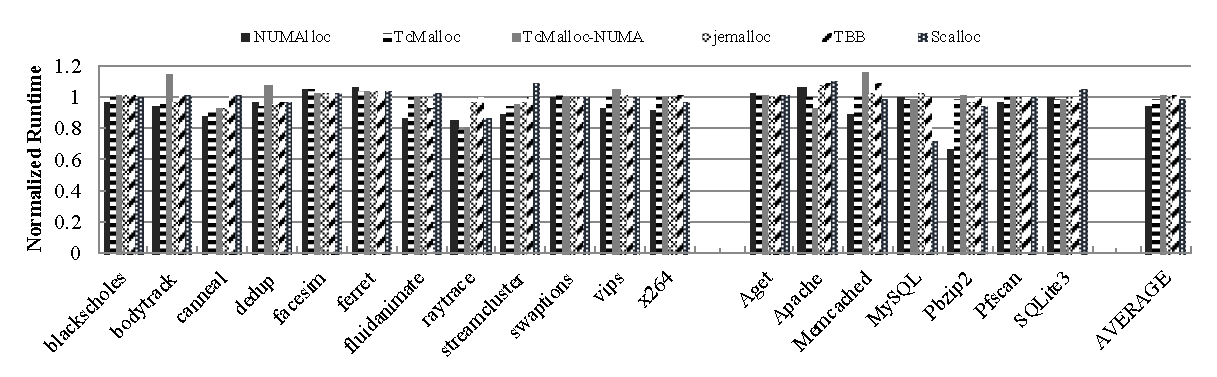
\includegraphics[width=\textwidth]{figure/2-node-parsec-perf.pdf}
   % \caption{Machine A (2-Node)\label{2node-parsec-perf}}
   % \end{subfigure}
    %\begin{subfigure}{0.9\textwidth}    
    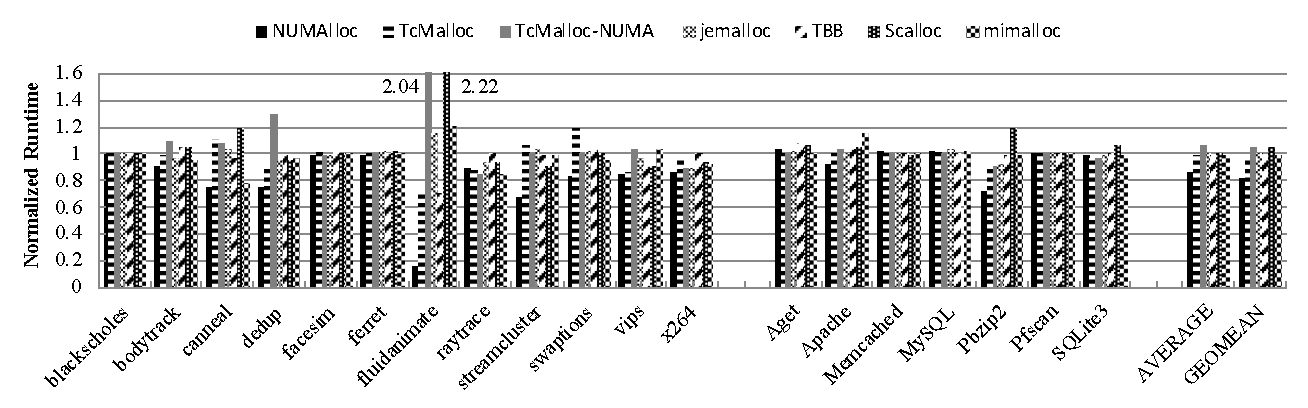
\includegraphics[width=5.2in]{figure/8-node-parsec-perf-new.pdf}
    %\caption{Machine B (8-Node)\label{8node-parsec-perf}}
    \caption{Performance of different allocators, where all data is normalized to that of the default Linux allocator. Here, a lower bar indicates a better performance.
    \label{fig:perf}}
 \end{figure*}

Overall, \NM{} has the best performance among these allocators. \NM{} is running 18.5\% faster than the default allocator, and 15.8\% faster than the second best one--TCMalloc~\cite{tcmalloc}, but does not run significantly slower than other allocators in almost all evaluated applications. For the best case (e.g., \texttt{fluidanimate}), \NM{} is running up to $6.4\times$ faster than the default Linux allocator, and it is $4.6\times$ than the second-best one--TCMalloc.  Comparing with the NUMA-aware allocator -- TCMalloc-NUMA~\cite{tcmallocnew}, \NM{} runs 23\% faster. The default Linux allocator achieves a good performance on the NUMA architecture due to its arena-based design, where each freed object will be returned back to its original arena.
This design is integrating well with Linux's first-touch allocation policy~\cite{Lameter:2013:NO:2508834.2513149} to ensure most thread-local allocations. 
In contrast, other allocators typically utilize a per-thread cache to store objects that are deallocated by the current thread, which may lead to remote accesses as described in Section~\ref{sec:intro}.  TCMalloc-NUMA and mimalloc are two allocators that are claimed to support the NUMA architecture among them~\cite{tcmallocnew}. But TCMalloc-NUMA's performance is even worse than that of TCMalloc. Based on our understanding, TCMalloc-NUMA is based on TCMalloc-0.97 (released in 2008), which does not have new features of TCMalloc-2.7 (the version for our evaluation). mimalloc only has the very basic NUMA support, which is the reason why it is not performing as well as \NM{}.  


Figure~\ref{fig:perf} shows that \NM{} has a similar or better performance than the default allocator in almost every application. Further, \NM{} has a significant performance improvement (over 20\%) in the following applications, including \texttt{canneal}, \texttt{dedup}, \texttt{fluidanimate}, \texttt{streamcluster}, and \texttt{pbzip2}. Among them, \NM{} has a super performance for \texttt{fluidanimate}, due to the following reasons. First, the interleaved heap contributes to $3.23\times$ performance speedup, as shown in Figure~\ref{fig:interleavedheap}. Second, node-balanced thread binding improves the performance by $4.45\times$. We further examine the number of remote accesses and TLB misses to confirm whether \NM{} significantly reduces them due to its design. 

We utilize the \texttt{perf} to collect the number of remote accesses and TLB misses (both load and store) on these applications when they are running with all allocators. 
%In our machine, we can collect these numbers using the following command: \texttt{perf stat -e node-load-misses,node-store-misses,dTLB-store-misses,dTLB-load-misses} 
The results are shown in Figure~\ref{fig:remoteAccess}. We combine the performance (shown as bars), remote accesses (red lines), and TLB misses (pin lines) together for a better comparison.   

Basically, \NM{} either significantly reduce the number of remote accesses or TLB misses, comparing to other allocators. That is the reason why it has much better performance on these applications. Let us utilize \texttt{fluidanimate} as an example. For remote accesses, the second best allocator (\texttt{TCMalloc}) has more than $5\times$ than \NM{}. We could see the similar results on TLB misses. \NM{}'s TLB misses is only 45\% of the second-best allocator (\texttt{mimalloc}). This explains why \NM{} is running up to $6.4\times$ faster than the default Linux allocator, and  $4.6\times$ than the second-best one--TCMalloc.


\begin{figure}[!h]
    \centering
    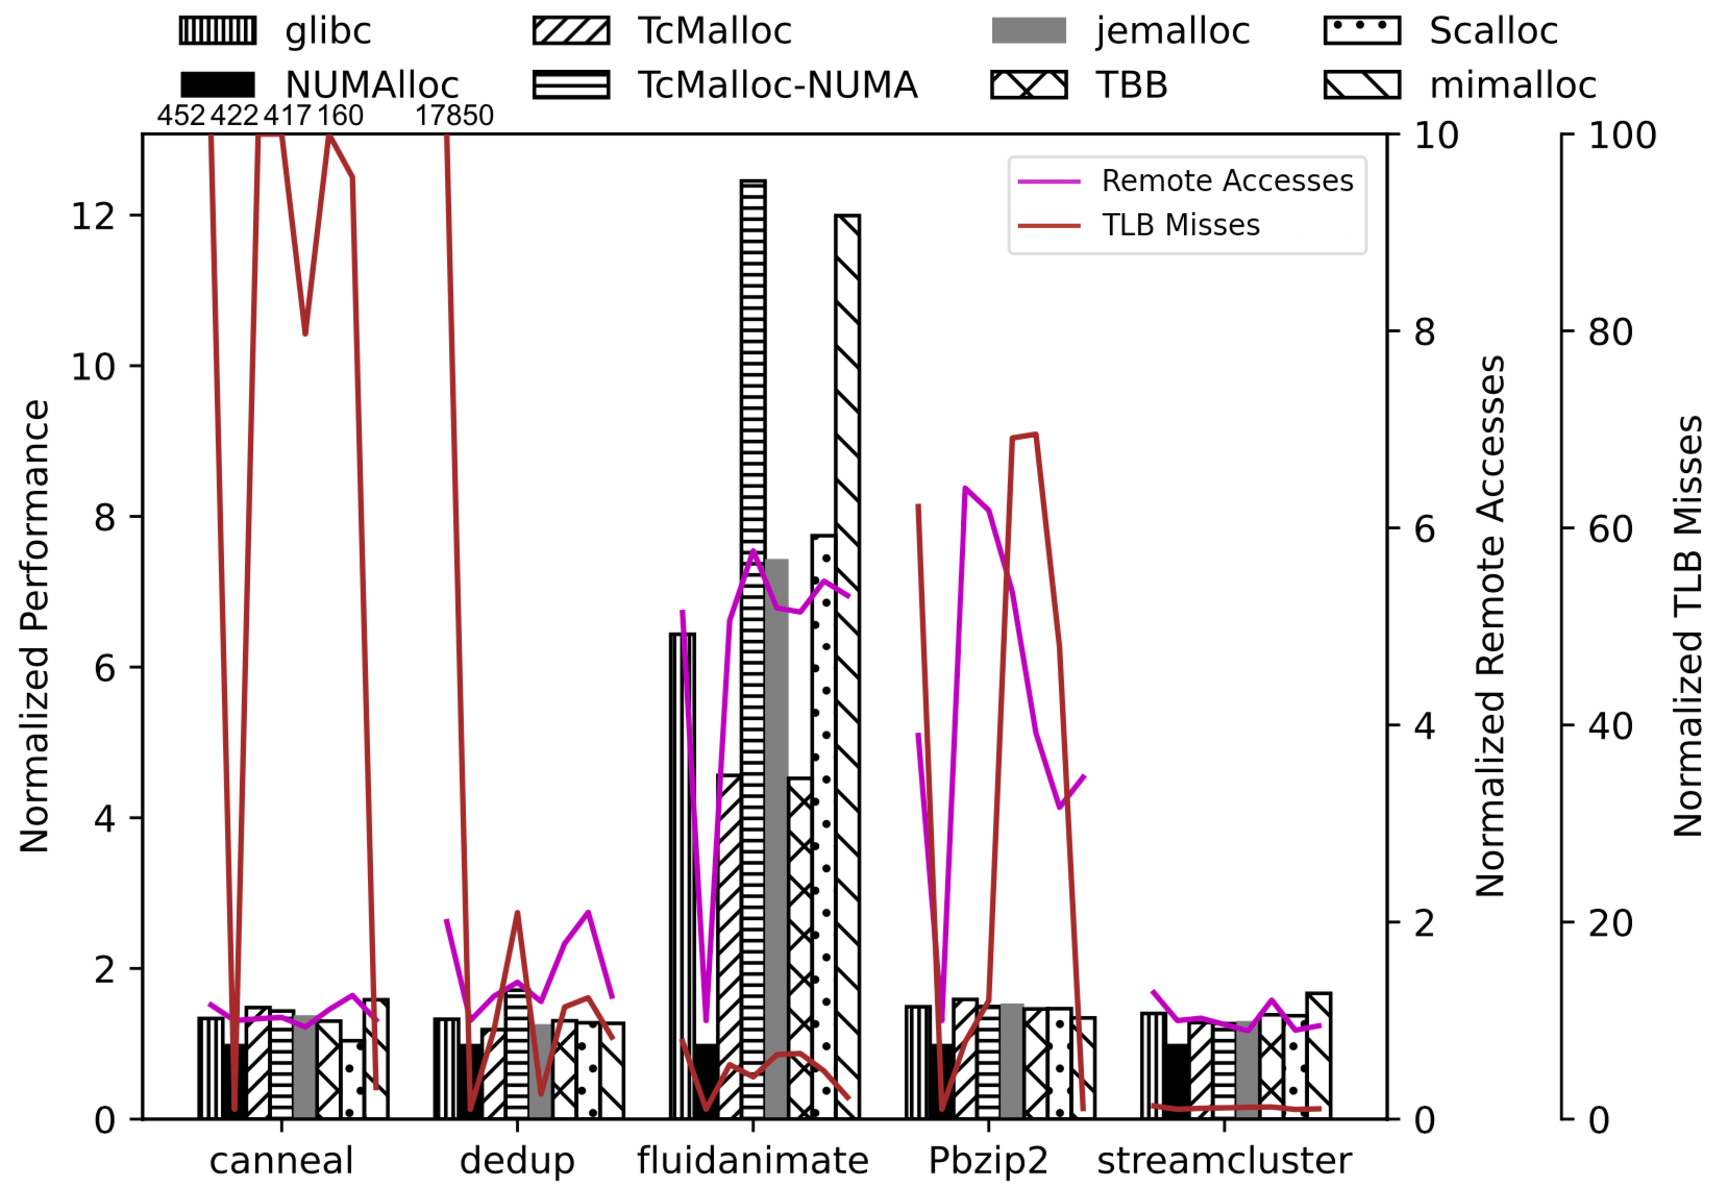
\includegraphics[width=3.5in]{figure/remote-access.pdf}
    \caption{Normalized remote access and TLB miss as well as normalized runtime, where all of them are normalized to \NM{}. }
    \label{fig:remoteAccess}
\end{figure}
\todo{Change "Performance" to runtime, also change the the performance/remote accesses" scale to 8, maybe put NUMAlloc to the first, change TcMalloc to TCMalloc. }

Based on our understanding, \NM{}'s big reduction of remote accesses can be attributed to the following factors: (1) region-based memory allocation; (2) (Node-balanced) thread binding; (3) Node-local meta data. The reduction of TLB misses can be possibly attributed to selective huge page support. Further, \NM{} allocates a large chunk of memory initially, then the OS tends to utilize huge pages if possible, although this mechanism may introduce more memory consumption as evaluated in Section~\ref{sec:memory}.  

\begin{comment}
\begin{table}[htp]
    \centering
    \footnotesize
    \begin{tabular}{l|c| c|c|c|c|c|c|c|c}
    \multicolumn{2}{c|}{Application} & glibc & \NM{} & TCM & TCM-NUMA & jemalloc & TBB & Scalloc & mimalloc \\ \hline
    \multirow{2}{*}{canneal} & Remote & 772 & 613 & 718   & 626 & 690 & 752 & 655 & 709\\ \cline{2-10}
    & TLB Misses &  & 975  &    &  &1876  & 1910 & 1836 & 1876 \\ \hline
    \multirow{2}{*}{dedup}  & Remote & 35.7 & 23.8 & 23.2 & 32.6 & & 29.9 & 28.4 & 23.7\\ \cline{2-10}
     & TLB &  & 21.6 &    &  & & 31.1 & 42.0  & 19.2\\ \hline
    \multirow{2}{*}{fluidanimate} & Remote  & 784 & 145 & 755 & 902 & & 741 & 798 & 749\\ \cline{2-10}
   & TLB  &  & 11.9  &    &  & & 116 & 137 & 100\\ \hline
    \multirow{2}{*}{streamcluster} & Remote  & 762 & 571 & 602 & 548 & & 768 & 497 & 570\\ \cline{2-10}
    &  TLB  &  & 12.1 &    &  & & 1455 & 1410 &  1432\\ \hline
    \multirow{2}{*}{pbzip2} & Remote  &  59.3 & 15.2 & 102 & 98.8 & & 62.5 & 45.8 & 60.4\\ \cline{2-10}
    & TLB &  & 0.8 &    &  & & 98.1 & 66.8 & 26.7 \\ \hline
    \end{tabular}
    \caption{TLB misses when using different allocators. The data shown is mega. }
    \label{tab:characteristics}
\end{table}

\end{comment}

%Table~\ref{tab:characteristics} shows that \NM{} significantly reduces the number of remote accesses and TLB misses due to its region-based design. 

%\todo{Hanmei: maybe we need to get the data on these applications. perf stat -e node-loads, node-load-misses, node-stores, node-store-misses ./APP a.out}



%We  can see that the average value of \NM{} is 0.97 in Machine A and 0.92 in Machine B and it is always the best among all other allocators. The reason that \NM{} got better performance in Machine B is that there are more nodes and more cores in Machine B, which means \NM{} could be very helpful to better to take use hardware resource of multi nodes and cores. but we could get amazing improvement if we shutdown interleaved heap in \NM{} and we will give the data in following sections.In the figure ~\ref{8node-parsec-perf}, we could see more exciting improvement from \NM{}, with average normalized value of 0.92 that is not only the best but also far aware better than all the rest allocators that TCMalloc and jemalloc got 0.99, TCMalloc-NUMA and TBB got roughly 1.07 and 1.01 separately. And also, we can see that the performance of \NM{} is the best for almost each single applications, especially it got 0.17 in fluidanimate and 0.66 in streamcluster which is far better than any of other allocators. As the same thing, the performance of ratrace and canneal is not good here, we will talk about it later after we shut down the interleaved heap.


%In the figure ~\ref{hoard-perf}, we show the normalized performance for Hoard benchmarks in Machine A and Machine B separately. We can see from figure ~\ref{hoard-perf} that the average value of \NM{} is also the best, which is 0.47 that means 2 times faster than default Linux Allocator, and jemalloc got 0.7 and Scalloc got 0.9. In the threadtest, the normalized value of \NM{} is 0.19 , far better than any of others, which means there are few central free list competitions, mainly contributed by properly node management and low overheads operations. For false sharing, \NM{}'s performance is also almost the best as same as Scalloc and jemalloc, which means they could handle false sharing issues very properly. In the larson, \NM{} and TCMalloc are the best, which mainly contributed by their low overheads for allocation and remote de-allocation, but due to our better node management, \NM{} could be better in the Machine B which will be mentioned later. In the figure ~\ref{hoard-perf}, we can also see that \NM{} got lowest average normalized value:0.33, significantly smaller than any of others that TBB got 0.99, Scalloc and jemalloc got roughly 1.14. And also, \NM{} and Scalloc could handle false sharing issue very well, and \NM{} could extremely well reduce central free list competition in threadtest. In larson, \NM{} is the best due to its properly multi-node management. 


\subsection{Memory Consumption}
\label{sec:memory}

We also measure the maximum memory consumption of these allocators. For non-server applications, such as \texttt{Aget}, \texttt{Pbscanf}, \texttt{Pbzip2} and all PARSEC applications, we utilized the sum of the \texttt{maxresident} output from the \texttt{time} utility and the size of huge pages, since the \texttt{time }output does not include huge pages. 
To determine the size of huge pages, a script is used to periodically collect the number of huge pages by reading from \texttt{/proc/meminfo} file, and then the maximum value of huge pages are used. 
For server applications, such as \texttt{MySQL}, \texttt{SQLite}, and \texttt{Memcached}, \texttt{Apache}, the maximum memory is collected by the sum of both \texttt{VmHWM} and \texttt{HugetlbPages} fields from \texttt{/proc/PID/status} file, after the corresponding client exits. 
%We always reboot server applications for each single test. 

%\end{comment}

% %\renewcommand{\arraystretch}{1.5}
\begin{table}[tp]
\footnotesize
	\setlength{\tabcolsep}{0.3em}
  \centering
    \begin{tabular}{|l|r|r|r|r|r|r|r|}
    \hline
    \multirow{2}{*}{Apps}&
    \multicolumn{7}{c|}{Memory Usage (MB)}\\
    \cline{2-8}
    &Linux&\NM{}&TcM&TcM-N&jem&TBB&Scalloc \\ \hline
    \hline
    blackscholes&615&509&621&623&633&615&630\\ \hline
    bodytrack&37&161&45&46&570&37&1994\\ \hline
    canneal&888&879&774&757&1294&888&36149\\ \hline
    dedup&912&1236&983&1023&1389&912&8556\\ \hline
    facesim&560&500&603&601&1133&547&3056\\ \hline
    ferret&184&493&195&183&596&184&3377\\ \hline
    fluidanimate&470&392&483&484&481&470&3437\\ \hline
    raytrace&1288&1472&1092&1543&1287&1288&4398\\ \hline
    streamcluster&113&105&123&121&127&113&193\\ \hline
    swaptions&33&268&16&21&540&37&1817\\ \hline
    vips&228&536&248&269&778&227&3681\\ \hline
    x264&2859&2721&3047&3064&3719&2859&5402\\ \hline \hline  
    Aget&8&74&11&10&93&8&80 \\ \hline
    Apache&8&34&10&9&10&4&42\\ \hline
    Memcached&16&80&25&24&41&18&263\\ \hline
    Mysql&277&732&314&315&500&276& N/A \\ \hline
    Pbzip2&463&747&817&813&1121&454&4881 \\ \hline
    Pfscan&522&542&528&528&535&522&554\\ \hline
    Sqlite3&45&284&60&75&139&44&681 \\ \hline
    \hline
    Total&{\bf 9527}&{\bf 11763}&{\bf 9993}&{\bf 10510}&{\bf 14986}&{\bf 9502}&{\bf 79190}\cr\hline
    \end{tabular}
  \caption{Memory consumption of different allocators. Here, TcM stands for TcMalloc, TcM-N is TcMalloc-NUMA, and jem is jemalloc. \label{tab:memory_consumption}}
\end{table}


Memory overhead is listed in Table~\ref{tab:memory_consumption}. In total, \NM{}'s memory consumption is around 45\% more than that of the default Linux allocator, but it is better than \texttt{jemalloc}, \texttt{mimalloc}, and \texttt{scalloc}.  The \texttt{glibc} allocator has the smallest memory consumption, and TCMalloc is the second-best one. 
%Scalloc is the worst one in terms of memory consumption, which consumes around  $8.3\times$ more memory that that of TBB.  
 
\NM{}'s more memory consumption is mainly due to the following reasons. \NM{} allocates a large memory block from the OS. When transparent huge page support is enabled, then all memory will be allocated from huge pages. The same reason also applies for Scalloc, which also allocates a continuous huge region of virtual memory from the underlying OS initially. We have confirmed that \NM{}'s memory overhead is very small, when transparent huge pages is disabled. Comparing to Scalloc, \NM{} makes all threads share the same bag for each size class, as described in Section~\ref{sec: others}, which effectively reduces its memory consumption by multiple times. In comparison, Scalloc utilizes $6\times$ more memory. Other allocators will not be affected by transparent huge pages, since they typically obtains a small chunk from the OS each time, less than the size of a huge page (2MB), then the OS will not allocate physical pages from huge pages by default.  
Therefore, we believe that \NM{}'s memory consumption is acceptable. 

%Second, \NM{} may not return the memory to the OS immediately for large pages. However, we believe that its memory consumption is acceptable. 
  %which actually shows the worst case for \NM{}. The OS will utilize huge pages if a memory area is larger than the size of a huge page (2MB). Since \NM{} utilizes \texttt{mmap} to allocate a huge chunk of virtual memory, this makes all heap memory for real objects will be allocated from huge pages. Currently, \NM{} also utilizes 1MB as the superblock for each size class, making objects of a size class that will occupy at least 1MB even if it only uses an object inside. 
 % Therefore, an application with many size classes will waste more memory. \NM{} makes all threads share the same bag for each size class, as described in Section~\ref{sec: others}, which effectively reduces its memory consumption by multiple times. 
 
 %Scalloc has excessive memory consumption, since its design does not support transparent huge pages very well. Similar to \NM{}, Scalloc utilizes a \texttt{mmap} system call to allocate a continuous huge region of virtual memory from the underlying OS. Since every thread will get a virtual span (2MB) for each size class in Scalloc, it will utilize 2MB physical memory even if only a word is touched. Differently, \NM{} avoids this issue as described in Section~\ref{sec: others}.
% the OS will assign a huge page when transparent huge page is enabled by default. Thus, if only one object is allocated from a size class, 
 
%\renewcommand{\arraystretch}{1.5}
\begin{table}[tp]
\footnotesize
	\setlength{\tabcolsep}{0.3em}
  \centering
    \begin{tabular}{|l|r|r|r|r|r|r|r|}
    \hline
    \multirow{2}{*}{Apps}&
    \multicolumn{7}{c|}{Memory Usage (MB)}\\
    \cline{2-8}
    &Linux&\NM{}&TcM&TcM-N&jem&TBB&Scalloc \\ \hline
    \hline
    blackscholes&615&509&621&623&633&615&630\\ \hline
    bodytrack&37&161&45&46&570&37&1994\\ \hline
    canneal&888&879&774&757&1294&888&36149\\ \hline
    dedup&912&1236&983&1023&1389&912&8556\\ \hline
    facesim&560&500&603&601&1133&547&3056\\ \hline
    ferret&184&493&195&183&596&184&3377\\ \hline
    fluidanimate&470&392&483&484&481&470&3437\\ \hline
    raytrace&1288&1472&1092&1543&1287&1288&4398\\ \hline
    streamcluster&113&105&123&121&127&113&193\\ \hline
    swaptions&33&268&16&21&540&37&1817\\ \hline
    vips&228&536&248&269&778&227&3681\\ \hline
    x264&2859&2721&3047&3064&3719&2859&5402\\ \hline \hline  
    Aget&8&74&11&10&93&8&80 \\ \hline
    Apache&8&34&10&9&10&4&42\\ \hline
    Memcached&16&80&25&24&41&18&263\\ \hline
    Mysql&277&732&314&315&500&276& N/A \\ \hline
    Pbzip2&463&747&817&813&1121&454&4881 \\ \hline
    Pfscan&522&542&528&528&535&522&554\\ \hline
    Sqlite3&45&284&60&75&139&44&681 \\ \hline
    \hline
    Total&{\bf 9527}&{\bf 11763}&{\bf 9993}&{\bf 10510}&{\bf 14986}&{\bf 9502}&{\bf 79190}\cr\hline
    \end{tabular}
  \caption{Memory consumption of different allocators. Here, TcM stands for TcMalloc, TcM-N is TcMalloc-NUMA, and jem is jemalloc. \label{tab:memory_consumption}}
\end{table}

 
\begin{comment}


In Figure~\ref{2node-hoard-mem}, the average normalized value of \NM{} is larger than others, but actually not too much, which is 2.3 for \NM{}, 1.9 for TCMalloc-NUMA and 1.8 for TCMalloc. It is because that proper node management is utilized in \NM{} and also in TCMalloc-NUMA, so that each node also preserves some memory not only thread locals.But we believe that this little more memory overheads are totally acceptable. It is also the same thing for Figure 10, that the average value for \NM{} is little higher than others, which is 5.3. But in this 8 nodes machine, numalloc is not the worst, that Scalloc's average value is 25 and jemalloc is 9.4. One main reason that the value of \NM{} is smaller is that we use mini size bags in \NM{} which is less than the size of one page for small objects and also memories for small objects are shared per node but per cores in Scalloc.
	
\end{comment}


\subsection{Scalability}
\label{sec:scale}

We also evaluated the scalability with four synthetic applications from Hoard~\cite{Hoard}, including \texttt{threadtest}, \texttt{larson}~\cite{Larson}, \texttt{cache-scratch} and \texttt{cache-slash}, which is also employed by existing work~\cite{Scalloc}. Among these applications, \texttt{larson} is to simulate a multithreaded server that could respond to requests from different clients, and \texttt{threadtest} is an application that performs a large number of allocations and deallocations within a specified number of threads. \texttt{cache-scratch} tests passive false sharing, and \texttt{cache-thrash} tests active false sharing. False sharing occurs when multiple threads are concurrently accessing different words in the same cache line. Passive false sharing is introduced upon deallocations, where a freed object can be utilized by another thread. In contrast, active false sharing is introduced during the initial allocations, where multiple continuous objects sharing the same cache line are allocated to different threads. The synthetic applications have a better scalability by design than other evaluated applications in the last section. 
%Since other allocators cannot specify the configuration, we only evaluate the scalability with different number of threads. 

In the evaluation, we maximize the number of threads on each node for \NM{}. For instance, the result of 32 threads will use 2 nodes, as each node has 16 cores. For other allocators, we only specify the number of threads, and it is up to the OS to perform the scheduling. The corresponding data is shown as Figure~\ref{sythentic-scalability}. All data are normalized to the data of one thread of the Linux's default allocator. 

\begin{figure*}[!th]
    \centering
    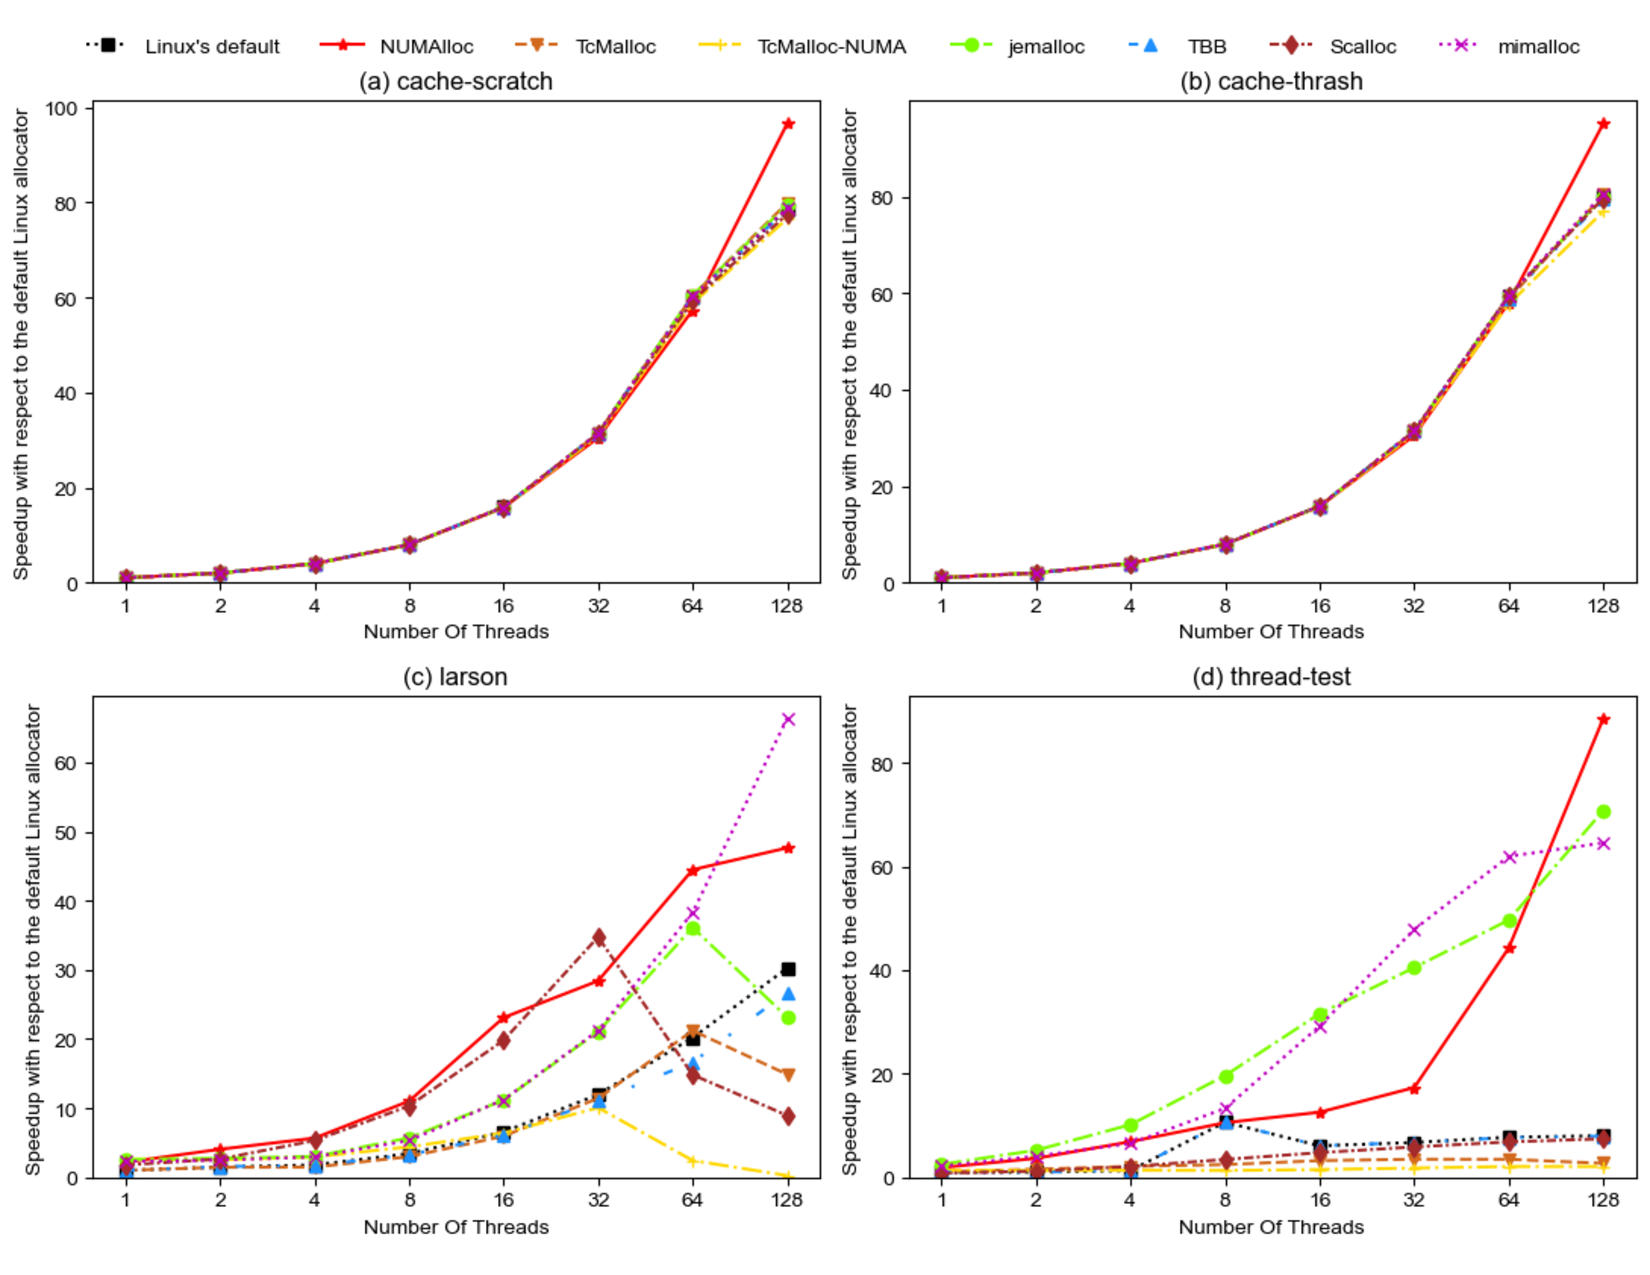
\includegraphics[width=\textwidth]{figure/sythentic-scalobility.pdf}
    \caption{Scalability of different allocators\\ all data is normalized to the runtime of the default Linux allocator with one thread.}
    \label{sythentic-scalability}
\end{figure*}

Overall, \NM{} has the best performance when the number of cores is 128. Its average speedup is $81\times$, comparing to the Linux's allocator with one thread, while the second best allocator--\texttt{mimalloc}-- has $72\times$ speedup. In contrast, the default Linux allocator only has the speedup of $49\times$. That is, \NM{} has the best scalability. When computing the speedup using the data of one thread of each allocator, \NM{}'s average speedup is $65\times$, while the second best one is $54\times$. All of these data indicates that \NM{} is scalable to 128 cores. 


%As shown in Figure~\ref{sythentic-scalability}, \NM{} has the best scalability than any other allocators, and has the best performance when the number of cores is 128, except for \texttt{larson}. \texttt{mimalloc} has a better throughput for this case. Overall, the performance speedup 

%However, comparing to \texttt{mimalloc}, \NM{} has much less memory consumption. Therefore, it is a clear better choice for the NUMA architecture. 


\begin{comment}

: 8 threads on one node (called as 8T1N), 16 threads on one node (16T1N) and two nodes (16T2N), 32 threads on two nodes (32T4N) and 4 nodes (32T4N), 64 threads on two nodes (64T4N) and 4 nodes (64T8N), and 128 threads on 8 nodes (128T8N). Machine B is chosen since it has more cores and more nodes, making it better to evaluate the scalability. \NM{}'s performance on these configurations is shown in Fig.~\ref{fig: numalloc-scalability}. For some applications, such as \texttt{facesim}, \texttt{ferret}, \texttt{fluidanimate}, \texttt{streamcluster}, \texttt{swaptions}, \NM{} scales very well. Some applications, such as \texttt{blackscholes}, \texttt{raytrace}, or \texttt{x264}, are not scalable very well.  We also observe that \NM{} typically performs better with the lower number of nodes, on a given number of threads.  This indicates that a lower number cores enables a better share of data among different threads. 

\begin{figure}[!h]
    \centering
    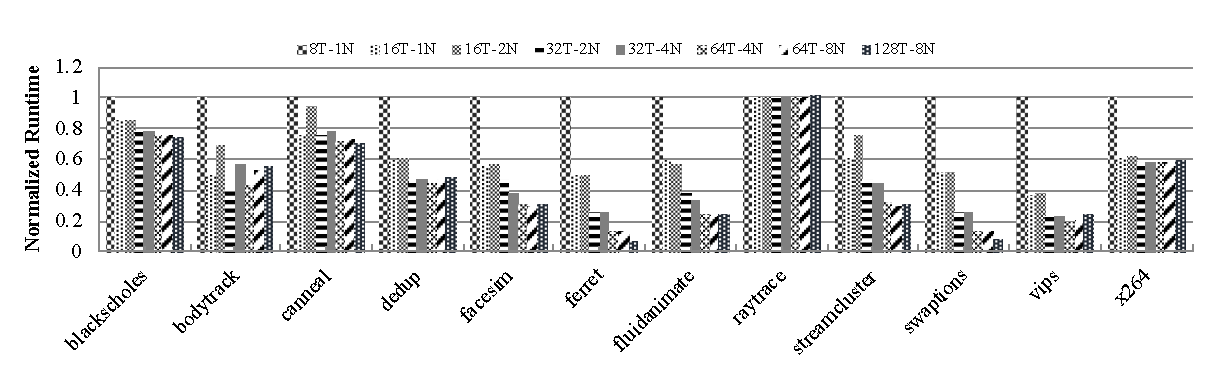
\includegraphics[width=\textwidth]{figure/scalobility-numalloc.pdf}
    \caption{Scalability of \NM{} with multiple configurations, where all data are normalized to runtime of 8T1N.\label{fig: numalloc-scalability}}
\end{figure}

\begin{figure}[!h]
    \centering
    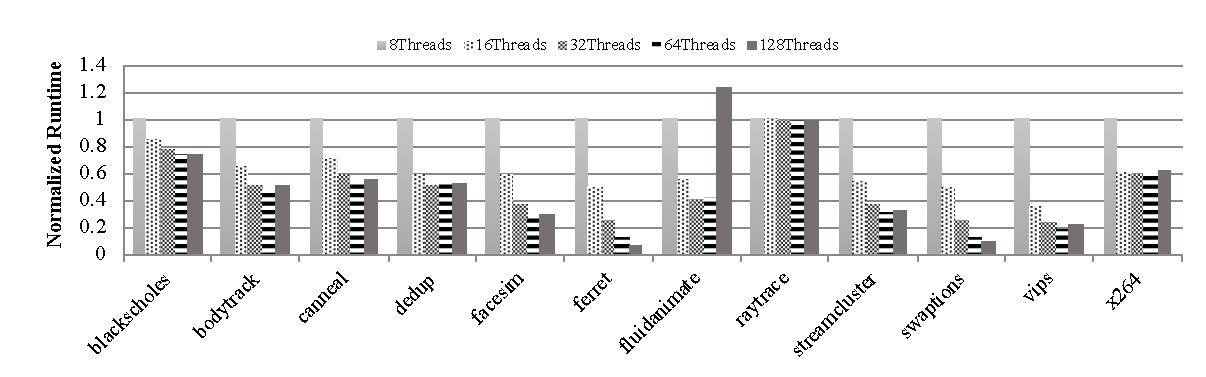
\includegraphics[width=\textwidth]{figure/scalability-pthread.pdf}
    \caption{Scalability of the Linux's default allocator, where all data are normalized to 8Threads.}
    \label{pthread-scalibity}
\end{figure}
	
\end{comment}

Among these applications, \texttt{cache-scratch} tests passive false sharing, and \texttt{cache-thrash} tests active false sharing. False sharing occurs when multiple threads are concurrently accessing different words in the same cache line. 
Passive false sharing is introduced upon deallocations, where a freed object can be utilized by another thread. In contrast, active false sharing is introduced during the initial allocations, where multiple continuous objects sharing the same cache line are allocated to different threads. 
%For these false sharing tests, we use 100,000 inner-loop, and 100,000 iterations with 8-byte objects.
 \NM{} will not introduce active false sharing, since each thread will get a page of objects initially. Although \NM{} might introduce passive false sharing due to its per-thread cache design, it avoids remote allocations across the node. 
 We believe that is the major reason for its better performance. Other allocators do not have such mechanisms. 
 That is the reason why \NM{} is one of the best allocators for \texttt{cache-scratch}, and achieves much better speedup than all other allocators in \texttt{cache-thrash} (30\% faster than the second-best one), as shown in Figure~\ref{sythentic-scalability}. TCMalloc has serious issues of both active and passive false sharing issue, which is the major reason that it does not perform well on these applications.  
 
 \texttt{larson} is to simulate a multithreaded server that could respond to requests from different clients. \NM{} is around 16\% faster than the second-best allocator--TCMalloc.  
 \texttt{threadtest} is an application that performs a large number of allocations and deallocations within a specified number of threads. \NM{} is $2.6\times$ faster than the second-best one (jemalloc), when there are 128 threads.
 %Each thread will receive a random number of objects in the beginning, perform a random number of allocation and deallocations to simulate the handler for processing requests, and then pass objects to the next thread. We test \texttt{larson} for 10 seconds with 1,000 objects for 10,000 iterations, where each allocation is between 7 bytes and 2048 bytes. 
 %As shown in Fig.~\ref{sythentic-scalability},  



%Also, it allows to specify how much work to be done between each allocation and deallocation. For \texttt{threadtest}, we use 100 iterations, 1,280,000 allocations, 0 work, and 64-byte objects (for the allocation).  This benchmark will stressfully test the performance overhead of allocation and deallocation. For this application, 
 %since every thread will has its own heap and it only imposes some when getting objects from the shared bag. But \NM{} obtains a number of objects at a time, at the page level, which significant reduce the possibility of contention. 


%On average,  \NM{} is running 79\% faster than the second-best one (Scalloc), and $2.2\times$ faster than the default Linux allocator. Multiple reasons contribute to the good performance of \NM{}: \NM{} imposes very minimal system call overhead, and little synchronization overhead. Also, it introduces less remote accesses than all other allocators, due to its NUMA-aware design. Other allocators have more or less false sharing issue, or incurs remote accesses.  
%\todo{Surprisingly, TCMalloc and  }.



%That is the reason why it has a good performance as the Linux allocator for \texttt{cache-thrash}.

 
\begin{comment}

\begin{figure}[!ht]
    \centering
    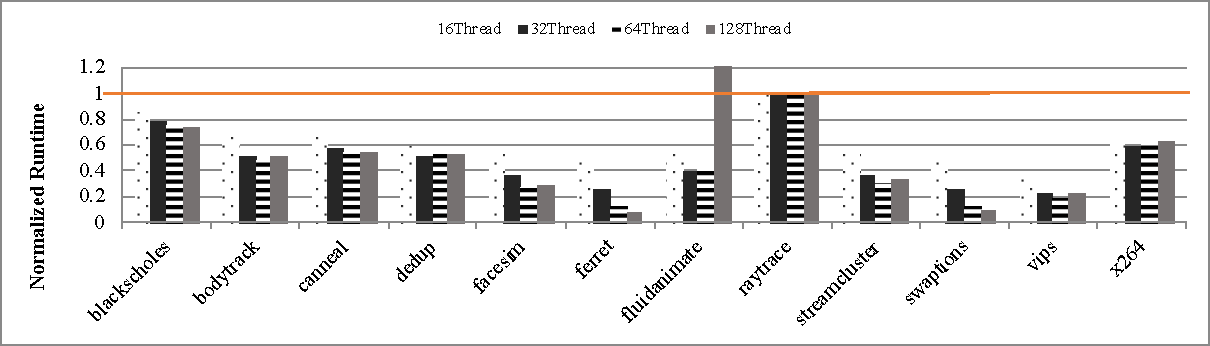
\includegraphics[width=\textwidth]{figure/scalobility-pthread.pdf}
    \caption{Normalized performance of Linux's default allocator without binding for PARSEC benchmarks in Machine B}
    \label{pthread-scalibity}
\end{figure}
We will evaluate the scalability on 8threads, 16threads, 32 threads, 64 threads and 128 threads. 
(one node, two node, four nodes, and 8 nodes). 
	
\end{comment}


\subsection{Design Choices}
\label{sec:design}

This section further confirms \NM{}'s multiple design choices, and all results shown in this section are normalized to the data of the default Linux allocator.  


%Based on our analysis, there are two reasons for this performance speedup. First, a thread will not be migrated to a different core, avoiding unnecessary remote accesses caused by cross-node migration, as further discussed in Section~\ref{sec:intro}. Second, \NM{}'s thread binding balances the workload, thus reducing the congestion of interconnect or one memory controller.


\subsubsection{Interleaved Heap} 
\label{sec:interleavedheap}

\begin{figure}[!h]
    \centering
    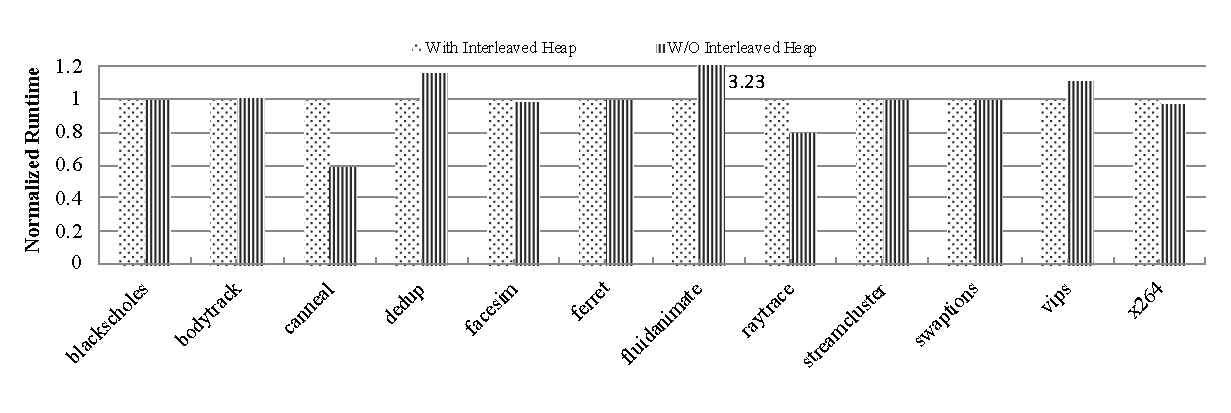
\includegraphics[width=3.2in]{figure/interleavedheap.pdf}
    \caption{Normalized runtime with and without  interleaved heap.\label{fig:interleavedheap}}  
\end{figure}

We also evaluate the potential benefit with the  interleaved heap. The performance data is shown as Figure~\ref{fig:interleavedheap}. Note that we have evaluated all real applications listed in Section~\ref{sec:performance}. The applications that have no or little performance impact by the interleaved heap are omitted in this figure. 

%\todo{Figure 7}
From Figure~\ref{fig:interleavedheap}, we have the following conclusion: the interleaved heap will benefit (or at least has no harmful impact on) the performance for most applications. Some applications, such as \texttt{fluidanimate}, will have the performance speedup of $3.23\times$ with the interleaved heap. However, applications having a large portion of time spent in the serial phase, such as \texttt{canneal} and \texttt{raytrace}, may not have good performance with the interleaved heap support. With the interleaved heap, \NM{} allocates the memory from all nodes interleavedly, instead of from the local node (based on the default first-touch policy). Therefore, private objects that are allocated in a remote node may introduce unnecessary overhead due to remote accesses.
 
Therefore, the interleaved heap will be enabled by default, unless programmers know that it will not benefit the performance. A simple metric is to use the portion of the serial phase inside a multithreaded applications.  That is, the interleaved heap will have a harmful impact on the serial execution, but may benefit the parallel execution because of its load balance. Therefore, programmers may turn off the interleaved heap for applications that are mostly running in serial phases. It is easy to turn on/off the interleved heap via a compilation flag or the environment variable.  

%, except applications with a large portion of serial phase (e.g., \texttt{canneal} and \texttt{raytrace})

%The interleaved heap could be utilized to avoid load imbalance issue for shared objets. 

%However, there are two issues for the interleaved heap. First, the allocator may not know whether an object is shared or not at the first time. Therefore, all objects that are allocated in the main heap (before creating any child thread) will be treated as the shared heap. Second, some applications are spending too much time in the serial phase, where the interleaved heap cannot benefit the performance for the serial phase. 


\subsubsection{Node-balanced Thread Binding}
\label{sec: threadbinding}

\begin{figure}[!h]
    \centering
    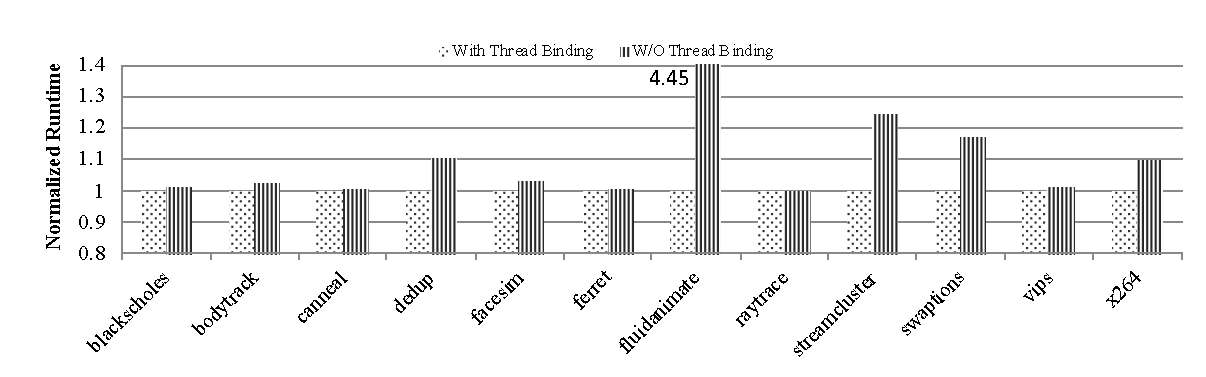
\includegraphics[width=3.2in]{figure/WO-pthread-binding.pdf}
    \caption{Normalized runtime with and without node-balanced thread binding}
    \label{binding-pthread-scalibity}
\end{figure}

Fig.~\ref{binding-pthread-scalibity} shows the performance difference with and without thread binding. Since \NM{} relies on thread binding that can not be disabled easily, we utilize the default Linux allocator to show the benefit with the node-balanced thread binding. Similarly, threads are bound to different nodes in a round-bin way. We observe that the thread binding improves the performance significantly for some applications. Among them, \texttt{fluidanimate} runs around $4.5\times$ faster with the thread binding, while \texttt{streamcluster} runs 22\% faster than the default one without the binding. This clearly indicates that the thread binding will benefit the performance overall. 


%figure ~\ref{parsec-no-interleaved-perf} we show some performance results of some applications that got significant different values after we shut down interleaved heap for \NM{}. We can see that for some applicatios with less data sharing between threads like ratrace and canneal, \NM{} could got significant improvements due to its low overheads and proper memory management. But for some other applications with intensive memory operations and sharing like fluidanimate, shutting down interleaved heap could hurt performance, since interleaved heap could help to distributed resource contention evenly over multi-nodes and then got low overheads.

\subsubsection{Selective Huge Pages} 
\label{sec:hugepage}

Since the machine utilizes transparent huge pages by default, we evaluate the performance impact of huge page support on another machine with 2 NUMA-node, without enabling the transparent huge pages.
% A, the 2-node machine. We only utilize PARSEC applications for this evaluation. 

\begin{figure}[!h]
    \centering
    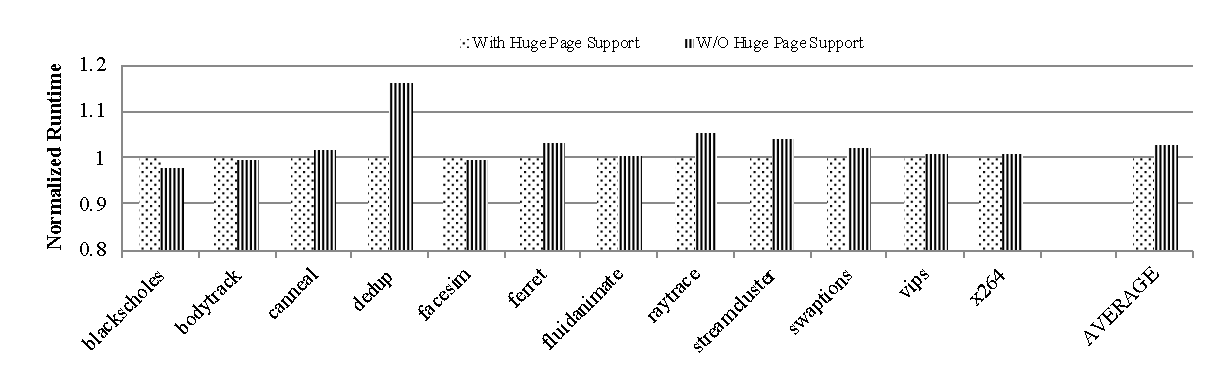
\includegraphics[width=3.2in]{figure/hugepage.pdf}
    \caption{Normalized runtime with and without selective huge pages.}
    \label{fig:hugepage}
\end{figure}

The results are shown in Figure~\ref{fig:hugepage}. When integrating with selective huge pages, \NM{} achieves a significantly better performance for \texttt{dedup}, where the performance difference is around 15\%. On average, the selective huge pages improves the performance of all evaluated applications about 2.5\%, and will not hurt the performance. This clearly indicates that it is beneficial to have selective huge pages for the NUMA architecture, especially given the fact of increasing memory size of hardware trend.  


